\chapter{Results}
\label{results}


\section{Implementation of the percolator algorithm}
- Reimplementierung funktioniert wie Original\\
- feature normalization war wichtiger boost\\
- ROC nach jeder Iteration zeigen

\section{Adapting Percolator to Cross-link Identification}
\label{lab:results:pseudo_rocs}
- Beispiel für ROCs nach jeder Iteration und wie die zu lesen sind (für alle, XLs und nXLs)
\subsection{Different Ranks}
\label{lab:results:ranks}
Figure~\ref{fig:before_optimalranking} shows the pseudo ROCs of Pycolator before the implementation of the new mechanism. \ref{fig:all_ranks} was plotted when Pycolator used all PSMs available, meaning all ranks, and only at the end lower ranking PSMs than 1 were excluded. \ref{fig:only_rank_one} is the result of running Pycolator only with rank 1 PSMs of the given dataset~\ref{lab:matmet:dataset} and~\ref{fig:optimalranking} shows the final result with the new feature.\\
As one can see, without the new mechanism Pycolator gradually improves the area under the curve and takes $5$ and $4$ iterations to roughly converge when given every PSM or only rank 1 PSMs to train respectively. This can be seen by the AUC results after every iteration or the ROC curves themselves. The end result, however, is better when removing the lower ranking PSMs right at the beginning (AUC of $345.79$) instead of in the end (AUC of $343.21$ after dropping the lower ranking PSMs). Since in the latter case Pycolator ended with an AUC of $343.79$ as one can see in~\ref{fig:all_ranks}, dropping the PSMs slightly worsened the end result. With the new feature, the algorithm takes about $5$ iterations to converge, then performs a jump and again improves over two iterations. The end result, an AUC of $348.13$, is higher than both alternatives. Multiple runs yielded very similar results. 
\renewcommand{\baselinestretch}{0.9}
\begin{figure}
	\normalsize
	\centering
	\begin{subfigure}{0.49\textwidth}
		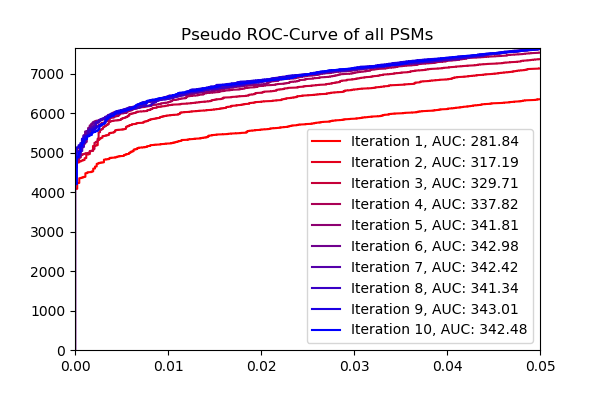
\includegraphics[width = \textwidth]{figures/allRanks.png}
		\caption[Result of dropping lower ranks at the end]{The resulting pseudo ROCs (explained in~\ref{lab:results:pseudo_rocs}) if Pycolator is given every PSM regardless of its rank. Lower ranking PSMs are only dropped in the end, which results in a final AUC of $343.21$.}
		\label{fig:all_ranks}
	\end{subfigure}
	\hfill
	\begin{subfigure}{0.49\textwidth}
		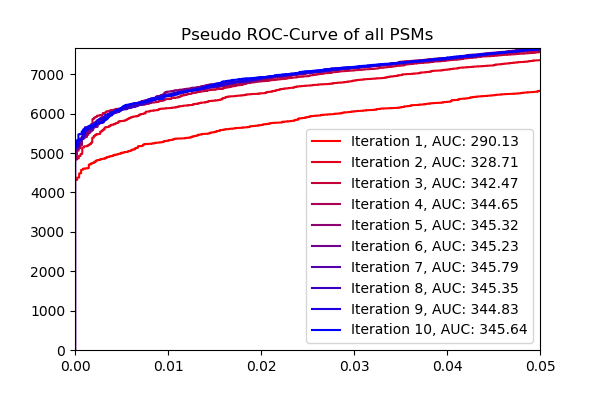
\includegraphics[width = \textwidth]{figures/onlyFirstRank.png}
		\caption[Result of dropping lower ranks at the start]{The resulting pseudo ROCs (explained in~\ref{lab:results:pseudo_rocs}) if Pycolator is given only the top scoring peptide for every spectrum. Lower ranking PSMs are dropped before running the algorithm.}
		\label{fig:only_rank_one}
	\end{subfigure}
	\begin{subfigure}{0.75\textwidth}
		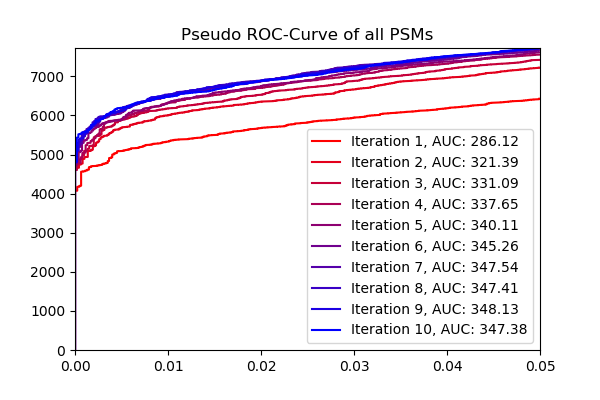
\includegraphics[width = \textwidth]{figures/optimalRanking.png}
		\caption[Result of the new ranking procedure]{The resulting pseudo ROCs (explained in~\ref{lab:results:pseudo_rocs}) if Pycolator is run with the newly implemented feature. It first trains with every PSM available, and after the results converge, lower ranking PSMs are dropped. Then, the algorithm runs for some more iterations.}
		\label{fig:optimalranking}
	\end{subfigure}
	\caption[Results of strategies regarding different ranks]{Results of running Pycolator with different strategies as to how lower ranking PSMs are dealt with.}
	\label{fig:before_optimalranking}
\end{figure}
\renewcommand{\baselinestretch}{1}

\subsection{Characteristics of Cross-linked PSMs}
\subsubsection{Proportions of Different Classes}
\label{lab:results:proportions}
- Verhältnis Targets:Decoys und XL:non-XL verringt die Streuung: MinMaxMedian Auswertungen\\
\subsubsection{Imputation}
\label{lab:results:imputation}
- Bei Imputation kam nichts heraus\\
\subsubsection{Splitting the Dataset}
\label{lab:results:splitting}
- Großer Unterschied wenn man den (großen) Datensatz nach XL/nXL oder sogar cross-linking target aufteilt\\

\subsection{Small datasets}
- Sinnvolle Plots zu Ratio Testing\\
- Neue Metrik erlaubt es der Implementierung, auch auf kleineren Datensätzen zu funktionieren